\section{Experiments}

\begin{frame}
	\frametitle{Experimental Evaluation}
	\framesubtitle{Environments}
	
	\vspace{-2.2cm}
	
	\Large
	
	\begin{figure}[!t]
		\centering
		\begin{tikzpicture}[map/.style={draw=black,ultra thick,inner sep=0pt}]
			\node at (-1,0) [map]
			{
				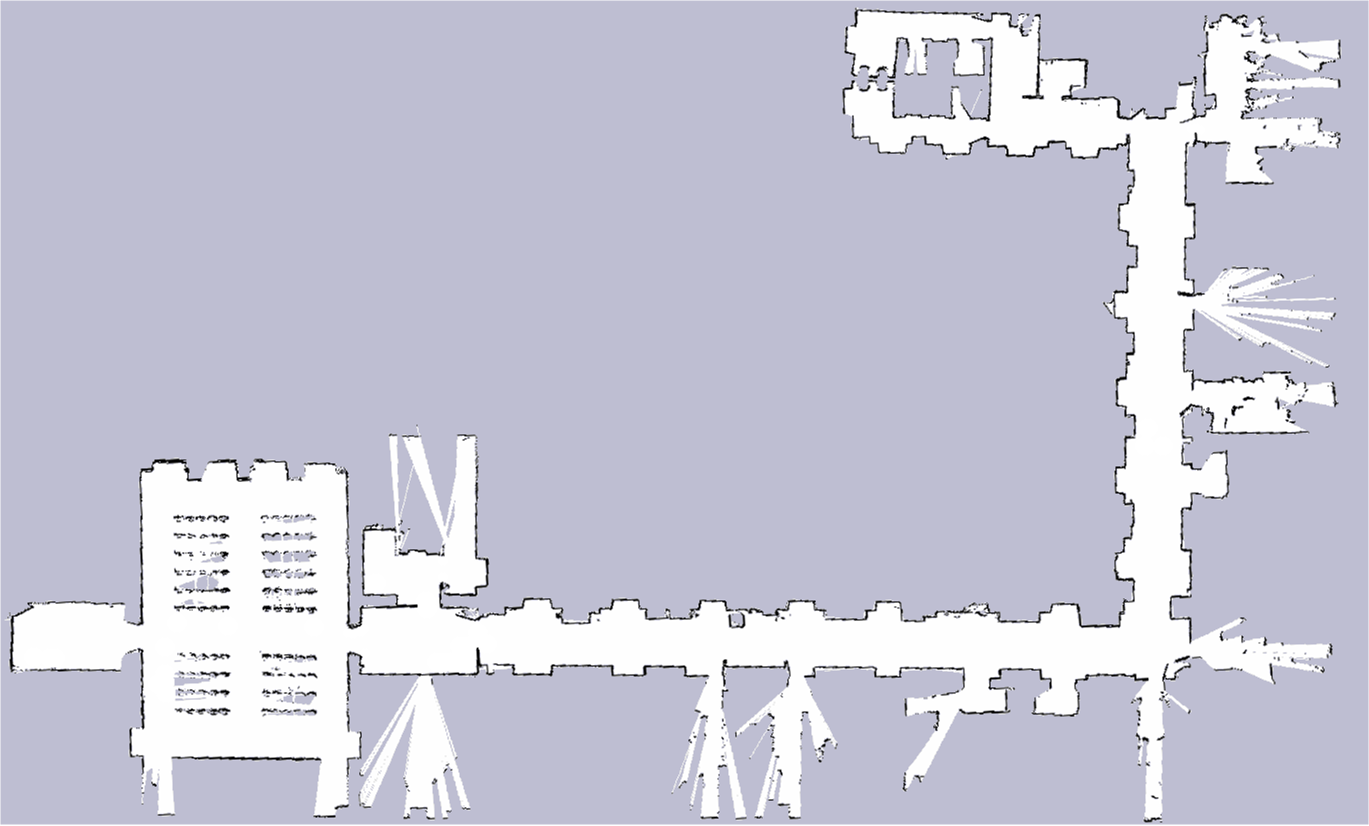
\includegraphics[width=5.9Cm]{Figures/Map-1}
			};
			\node at (5.1,-2.7) [map]
			{
				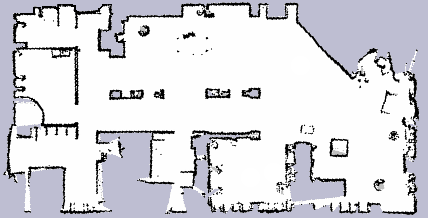
\includegraphics[width=5.9cm]{Figures/Map-2}
			};
		\end{tikzpicture}
	\end{figure}
	
	\vspace{-3.3cm}
	
	\begin{tabbing}
		\hspace{2.15cm}
		\textbf{DIAG}
	\end{tabbing}
	
	\vspace{-2.95cm}
	
	\begin{tabbing}
		\hspace{7.35cm}
		\textbf{Peccioli House}
	\end{tabbing}
\end{frame}

\begin{frame}
	\frametitle{Experimental Evaluation}
	\framesubtitle{Problem modeling}
	
	\Large
	
	\vspace{0.3cm}
	
	The problem of monitoring a populated environment can be modeled as a \textbf{Prey-Predator}
	game.
	
	\vspace{0.3cm}
	
	We can consider sensor nodes as \emph{predators} and the moving objects to be monitored as
	\emph{preys}
	
	\vspace{-0.5cm}
	
	\begin{center}
		\Huge
		\textcolor{blue}{$ \Downarrow $}
	\end{center}
	
	\vspace{-0.5cm}
	
	\begin{block}{Prey-Predator Game}
		\emph{A predator tries to catch preys and a prey runs away from predators}
	\end{block}
\end{frame}

\begin{frame}
	\frametitle{Experimental Evaluation}
	\framesubtitle{Evaluation Metrics - Tracking}
	
	\Large
	
	\vspace{0.5cm}
	
	\emph{Multiple Object Tracking Accuracy} (\emph{MOTA}) is defined as:
	
	\vspace{-0.5cm}
	
	\begin{equation*}
		MOTA = 1 - \frac{\sum_{t=1}^{N_{frames}} (c_m(m_t) + c_f(fp_t) + cs(ID\mbox{-}S_t))}{\sum_{t=1}^{N_{frames}} N_G^{(t)}}
	\end{equation*}
	
	\vspace{0.4cm}
	
	\emph{Multiple Object Tracking Precision} (\emph{MOTP}) is defined as:
	
	\vspace{-0.1cm}
	
	\begin{equation*}
		MOTP = \frac{\sum_{i=1}^{N_{mapped}} \sum_{t=1}^{N_{frames}^{(t)}} \Big [ \frac{| G_i^{(t)} \cap D_i^{(t)} |}{| G_i^{(t)} \cup D_i^{(t)} |} \Big ] }{\sum_{t=1}^{N_{frames}} N_{mapped}^{(t)}}
	\end{equation*}
\end{frame}

\begin{frame}
	\frametitle{Experimental Evaluation}
	\framesubtitle{Evaluation Metrics - Integrated System}
	
	\Large
	
	\vspace{0.5cm}
	
	Mean distance between robots and moving objects is computed as follows:
	
	\vspace{-0.4cm}
	
	\begin{equation*}
		avg = \sum_{t=1}^n \sum_{i=1}^k \frac{1}{k} \frac{\sum_{j=1}^m \| e_{i,j}^{(t)} - g_{j}^{(t)} \|}{m}
	\end{equation*}
	
	\vspace{0.4cm}
	
	while the deviation standard as follows:
	
	\vspace{-0.3cm}
	
	\begin{equation*}
		std. \; dev. = \sum_{t=1}^n \sum_{i=1}^k \frac{1}{k} \frac{\sum_{j=1}^m \| e_{i,j}^{(t)} - avg_{i}^{(t)} \|}{m}
	\end{equation*}
\end{frame}

\begin{frame}
	\frametitle{Experimental Evaluation}
	\framesubtitle{Setup}
	
	\Large
	
	\vspace{0.2cm}
	
	Same set of sensor's configuration for both scenarios:
	
	\begin{itemize}
		\item \textbf{Setting 1:} 3 fixed cameras, no robots with cameras
		
		\item \textbf{Setting 2:} 2 fixed cameras, 1 robot with a camera
		
		\item \textbf{Setting 3:} 1 fixed camera, 2 robots with a camera
		
		\item \textbf{Setting 4:} 3 robots with a camera
	\end{itemize}
	
	\vspace{-0.5cm}
	
	\begin{columns}[T]
		\column{.95\textwidth}
		
		\begin{block}{Goal}
			Show the benefits of having a mobile sensor close to an object rather than having
			a set of fixed sensors with a high probability to provide unreliable information
		\end{block}
	\end{columns}
\end{frame}

\begin{frame}
	\frametitle{Experimental Evaluation}
	\framesubtitle{Artificial Noise}
	
	\large
	
	\vspace{0.3cm}
	
	\begin{enumerate}
		\item \textbf{Sensor accuracy:} observations provided by the sensor within a range of
			  $ 5 $ $ m $ are linearly degraded, while the further ones will degrade
			  quadratically with respect to the object distance
		\vspace{0.1cm}
		\item \textbf{Localization error: } additional localization error within $ [8,16] $
			  $ cm $ has been added to the mobile sensor node
		\vspace{0.1cm}
		\item \textbf{Network reliability:} a message is lost with a probability $ 0.15 $,
			  delayed with a probability $ 0.25 $ or delivered with a probability $ 0.6 $.
			  Moreover, network could be unavailable - for a robot - with a probability $ 0.3 $
			  for a temporal window within $ (0,5] $ seconds
		\vspace{0.1cm}
		\item \textbf{Limited communication range:} robots communicate their information within
			  a $ 5m $ communication range due to a simulated wireless network
	\end{enumerate}
\end{frame}

\begin{frame}
	\frametitle{Experimental Evaluation}
	\framesubtitle{Results - DIAG}
	
	\footnotesize
	
	\vspace{0.3cm}
	
	\begin{table}[!t]
		\centering
		\begin{tabular}{ccccc}
			\cline{1-5}
			\multicolumn{1}{l}{} & \multicolumn{4}{c}{\textbf{\begin{tabular}[c]{@{}c@{}}Prey-Predator Distance\\ (avg $ \pm $ std. dev.)\end{tabular}}} \\ \hline
			\multicolumn{1}{c}{\textbf{\#}} & \textbf{Setting 1} & \textbf{Setting 2} &
			\textbf{Setting 3} & \textbf{Setting 4} \\
			
			\multicolumn{1}{c}{1} & 3.04 $ m $ $ \pm $ 0.63 $ m $ & 2.70 $ m $ $ \pm $ 0.49 $ m $
								  & 2.02 $ m $ $ \pm $ 0.38 $ m $ & 1.12 $ m $ $ \pm $ 0.19 $ m $ \\
			\multicolumn{1}{c}{2} & 2.95 $ m $ $ \pm $ 0.80 $ m $ & 2.65 $ m $ $ \pm $ 0.48 $ m $
								  & 1.95 $ m $ $ \pm $ 0.42 $ m $ & 1.15 $ m $ $ \pm $ 0.20 $ m $ \\
			\multicolumn{1}{c}{3} & 3.12 $ m $ $ \pm $ 0.53 $ m $ & 2.87 $ m $ $ \pm $ 0.56 $ m $
								  & 2.03 $ m $ $ \pm $ 0.41 $ m $ & 1.13 $ m $ $ \pm $ 0.19 $ m $ \\
			\multicolumn{1}{c}{4} & 3.01 $ m $ $ \pm $ 0.69 $ m $ & 2.73 $ m $ $ \pm $ 0.49 $ m $
								  & 2.06 $ m $ $ \pm $ 0.38 $ m $ & 1.08 $ m $ $ \pm $ 0.22 $ m $ \\
			\multicolumn{1}{c}{5} & 2.99 $ m $ $ \pm $ 0.72 $ m $ & 2.86 $ m $ $ \pm $ 0.61 $ m $
								  & 1.99 $ m $ $ \pm $ 0.40 $ m $ & 1.11 $ m $ $ \pm $ 0.17 $ m $ \\
								  \cline{1-5}
		\end{tabular}
	\end{table}
	
	\vspace{-0.2cm}
	
	\begin{table}[!t]
		\centering
		\begin{tabular}{ccccc}
			\cline{1-5}
			\multicolumn{1}{l}{} & \multicolumn{4}{c}{\textbf{\begin{tabular}[c]{@{}c@{}}Tracking Performance\\ (MOTA,MOTP)\end{tabular}}} \\ \hline
			\multicolumn{1}{c}{\textbf{\#}} & \textbf{Setting 1} & \textbf{Setting 2} &
			\textbf{Setting 3} & \textbf{Setting 4} \\
			
			\multicolumn{1}{c}{1} & (0.63,0.45) & (0.67,0.49) & (0.75,0.51) & (0.94,0.75) \\
			\multicolumn{1}{c}{2} & (0.59,0.42) & (0.65,0.45) & (0.73,0.49) & (0.92,0.74) \\
			\multicolumn{1}{c}{3} & (0.64,0.41) & (0.69,0.48) & (0.70,0.47) & (0.95,0.77) \\
			\multicolumn{1}{c}{4} & (0.62,0.45) & (0.62,0.40) & (0.74,0.50) & (0.92,0.75) \\
			\multicolumn{1}{c}{5} & (0.57,0.39) & (0.64,0.44) & (0.70,0.48) & (0.94,0.77) \\ \cline{1-5}
		\end{tabular}
	\end{table}
\end{frame}

\begin{frame}
	\frametitle{Experimental Evaluation}
	\framesubtitle{Results - Peccioli House}
	
	\footnotesize
	
	\vspace{0.3cm}
	
	\begin{table}[!t]
		\centering
		\begin{tabular}{ccccc}
			\cline{1-5}
			\multicolumn{1}{l}{} & \multicolumn{4}{c}{\textbf{\begin{tabular}[c]{@{}c@{}}Prey-Predator Distance\\ (avg $ \pm $ std. dev.)\end{tabular}}} \\ \hline
			\multicolumn{1}{c}{\textbf{\#}} & \textbf{Setting 1} & \textbf{Setting 2} &
			\textbf{Setting 3} & \textbf{Setting 4} \\
			
			\multicolumn{1}{c}{1} & 2.84 $ m $ $ \pm $ 0.59 $ m $ & 2.55 $ m $ $ \pm $ 0.47 $ m $
								  & 1.85 $ m $ $ \pm $ 0.38 $ m $ & 1.07 $ m $ $ \pm $ 0.18 $ m $ \\
			\multicolumn{1}{c}{2} & 2.85 $ m $ $ \pm $ 0.74 $ m $ & 2.52 $ m $ $ \pm $ 0.51 $ m $
								  & 1.84 $ m $ $ \pm $ 0.40 $ m $ & 1.05 $ m $ $ \pm $ 0.21 $ m $ \\
			\multicolumn{1}{c}{3} & 3.03 $ m $ $ \pm $ 0.57 $ m $ & 2.76 $ m $ $ \pm $ 0.52 $ m $
								  & 1.91 $ m $ $ \pm $ 0.43 $ m $ & 1.11 $ m $ $ \pm $ 0.20 $ m $ \\
			\multicolumn{1}{c}{4} & 3.04 $ m $ $ \pm $ 0.61 $ m $ & 2.63 $ m $ $ \pm $ 0.47 $ m $
								  & 1.93 $ m $ $ \pm $ 0.39 $ m $ & 1.08 $ m $ $ \pm $ 0.21 $ m $ \\
			\multicolumn{1}{c}{5} & 2.89 $ m $ $ \pm $ 0.68 $ m $ & 2.77 $ m $ $ \pm $ 0.56 $ m $
								  & 1.89 $ m $ $ \pm $ 0.41 $ m $ & 1.09 $ m $ $ \pm $ 0.15 $ m $ \\
								  \cline{1-5}
		\end{tabular}
	\end{table}
	
	\vspace{-0.2cm}

	\begin{table}[!t]
		\centering
		\begin{tabular}{ccccc}
			\cline{1-5}
			\multicolumn{1}{l}{} & \multicolumn{4}{c}{\textbf{\begin{tabular}[c]{@{}c@{}}Tracking Performance\\ (MOTA,MOTP)\end{tabular}}} \\ \hline
			\multicolumn{1}{c}{\textbf{\#}} & \textbf{Setting 1} & \textbf{Setting 2} &
			\textbf{Setting 3} & \textbf{Setting 4} \\
			
			\multicolumn{1}{c}{1} & (0.67,0.42) & (0.71,0.49) & (0.78,0.58) & (0.93,0.79) \\
			\multicolumn{1}{c}{2} & (0.62,0.43) & (0.69,0.46) & (0.77,0.55) & (0.95,0.76) \\
			\multicolumn{1}{c}{3} & (0.64,0.47) & (0.73,0.51) & (0.72,0.52) & (0.96,0.79) \\
			\multicolumn{1}{c}{4} & (0.66,0.44) & (0.68,0.43) & (0.75,0.53) & (0.93,0.77) \\
			\multicolumn{1}{c}{5} & (0.60,0.41) & (0.65,0.45) & (0.71,0.51) & (0.97,0.81) \\ \cline{1-5}
		\end{tabular}
	\end{table}
\end{frame}
